\documentclass[a4paper]{article}

\usepackage{INTERSPEECH2016}

\usepackage{graphicx}
\graphicspath{ {../} }
\usepackage{amssymb,amsmath,bm,bbm}
\usepackage{hyperref}
\usepackage{textcomp}
\usepackage{algorithm}
\usepackage{algpseudocode}
\usepackage{array}
\usepackage{multirow}
\usepackage[caption=false,font=footnotesize]{subfig}

\def\vec#1{\ensuremath{\bm{{#1}}}}
\def\mat#1{\vec{#1}}
\DeclareMathOperator{\round}{round}
\DeclareMathOperator{\elbo}{ELBO}
\DeclareMathOperator{\bce}{BCE}
\DeclareMathOperator{\unif}{Unif}
\DeclareMathOperator{\cov}{Cov}

\sloppy % better line breaks
\ninept

\title{Query Selection based on Latent Space Sampling}

%%%%%%%%%%%%%%%%%%%%%%%%%%%%%%%%%%%%%%%%%%%%%%%%%%%%%%%%%%%%%%%%%%%%%%%%%%
%% If multiple authors, uncomment and edit the lines shown below.       %%
%% Note that each line must be emphasized {\em } by itself.             %%
%% (by Stephen Martucci, author of spconf.sty).                         %%
%%%%%%%%%%%%%%%%%%%%%%%%%%%%%%%%%%%%%%%%%%%%%%%%%%%%%%%%%%%%%%%%%%%%%%%%%%
%\makeatletter
%\def\name#1{\gdef\@name{#1\\}}
%\makeatother
%\name{{\em Firstname1 Lastname1, Firstname2 Lastname2, Firstname3 Lastname3,}\\
%      {\em Firstname4 Lastname4, Firstname5 Lastname5, Firstname6 Lastname6,
%      Firstname7 Lastname7}}
%%%%%%%%%%%%%%% End of required multiple authors changes %%%%%%%%%%%%%%%%%

\makeatletter
\def\name#1{\gdef\@name{#1\\}}
\makeatother \name{{\em Benjamin Killeen}}

\address{University of Chicago \\
  {\small \tt killeen@uchicago.edu}
}

\begin{document}
\maketitle

\begin{abstract}
  The advent of deep learning has facilitated remarkable success on increasingly
  complex tasks. Large datasets are integral to this success, providing example
  labels which guide training, but many tasks are unrelated to existing
  datasets. In these cases, the choice of an \emph{initial query set} for
  annotation is crucial. A well-sampled query set can facilitate downstream
  approaches like semi-supervised or active learning, both of which require a
  small, labeled dataset. In this paper, we focus on sampling strategies using
  latent-space representations learned by auto-encoders, a self-supervised
  variant of deep neural networks. Furthermore, we constrain our latent-space to
  just two dimensions. Although potentially limiting, this focus allows for an
  easy visualization of latent spaces well-suited for initial exploration of the
  topic. We evaluate each sampling strategy using a simple classifier trained on
  just the initial query set.\footnote{Code and additional figures available at
    \href{https://github.com/bendkill/latens}{github.com/bendkill/latens}.}
\end{abstract}
\noindent{\bf Index Terms}: semi-supervised learning, active learning, computer
vision

\section{Introduction}
\label{sec:introduction}

% relevance of selecting a 
The collection and annotation of large datasets has been critical to the success
of deep learning. Wherever such data is available, it seems, the focus of the
community eventually results in an effective design for a supervised
model. Although that model's performance may extend to similar tasks, many
application domains exist outside the scope of established datasets. This is the
case especially for scientific image analysis, where the unique nature of each
experiment sets it apart from conventional tasks and obtaining labels can
require significant investment, monetary- or labor-wise, due to task
complexity. Object detection, for instance, requires more in-depth annotation
than simple classification. In general, these scenarios call for an approach
that minimizes the labeling required to learn a specific task, starting from
scratch.

% discuss downstream approaches this is suitable for
Several sub-fields of machine learning confront this challenge. An active
learning approach, firstly, iteratively selects new examples for labeling in the
hopes of improving model performance at every step \cite{settles_active_2012}. A
popular sampling strategy incorporates the uncertainty of the model for each
unlabeled example \cite{settles_active_2012, lewis_sequential_1994}. Here, the
\emph{initial query set} is used to train the first iteration of the model,
before any active learning can take place. Typically, the initial query set is
selected randomly. This works well in many cases, but we hypothesize that a
well-sampled initial query set would result in a better initial model,
accelerating the active learning process. Although such tests are beyond the
scope of this paper, they remain an active area of inquiry. Secondly, a
semi-supervised approach, uses both labeled and unlabeled data during training
\cite{zhu_semi-supervised_2005}. Since the initial query set is actually the
\emph{only} query set, a well-sampled training set is of the utmost importance
for semi-supervised learning.

% define metric for success
At this point, the meaning of ``well-sampled'' is, admittedly, not readily
apparent. One would hope, for instance, that a well-sampled query set contains
instances from every class, in the case of classification, or from a wide range
of values, in the case of regression. Moreover, the representation of these
classes or values seemingly ought to be well-balanced, as if sampled
\emph{i.i.d.} not from the larger data, which may contain biases, but from the
natural distribution itself. However, these properties, however, are distinctly
qualitative. One way to quantitatively evaluate the quality of a sampling would
be through the performance of a downstream approach that uses an initial query
set, such as semi-supervised or active learning. In our experiments, we choose a
much simpler downstream approach, namely using the initial query set as the sole
training set for a simple classifier. The accuracy of this classifier, measured
on a withheld test set, serves as our measure for the ``well-sampled-ness'' of a
query set.

% narrow down to what this paper actually does (needs more work)
In this paper, we focus on sampling strategies that rely on a latent space
representation of the unlabeled set. In particular, we explore latent spaces
learned by an auto-encoder (AE) because of the opportunity for similar network
design \cite{goodfellow_deep_nodate}. Our sampling strategies, meanwhile,
attempt to approximate a probability distribution in the latent space. There are
many choices of AE and distribution; here, we present several options that
illustrate the properties of each representation.

\section{Related Work}
\label{sec:related-work}

We draw on numerous works for guidance. We are inspired, firstly, by the
potential for well-sampled initial query sets in the areas of active and
semi-supervised learning, sub-fields of machine learning laid out by Settles
\emph{et al.} and Zhu, respectively \cite{settles_active_2012,
  zhu_semi-supervised_2005}. We draw form Krixhevsky \emph{et al.} for the
design of our convolutional AE, as well as on the work of Kingman \emph{et al.}
and Maaten \emph{et al.} for their work on variational auto-encoders and t-SNE
embeddings, respectively.

\section{Method}
\label{sec:method}

\begin{figure}
  \centering
  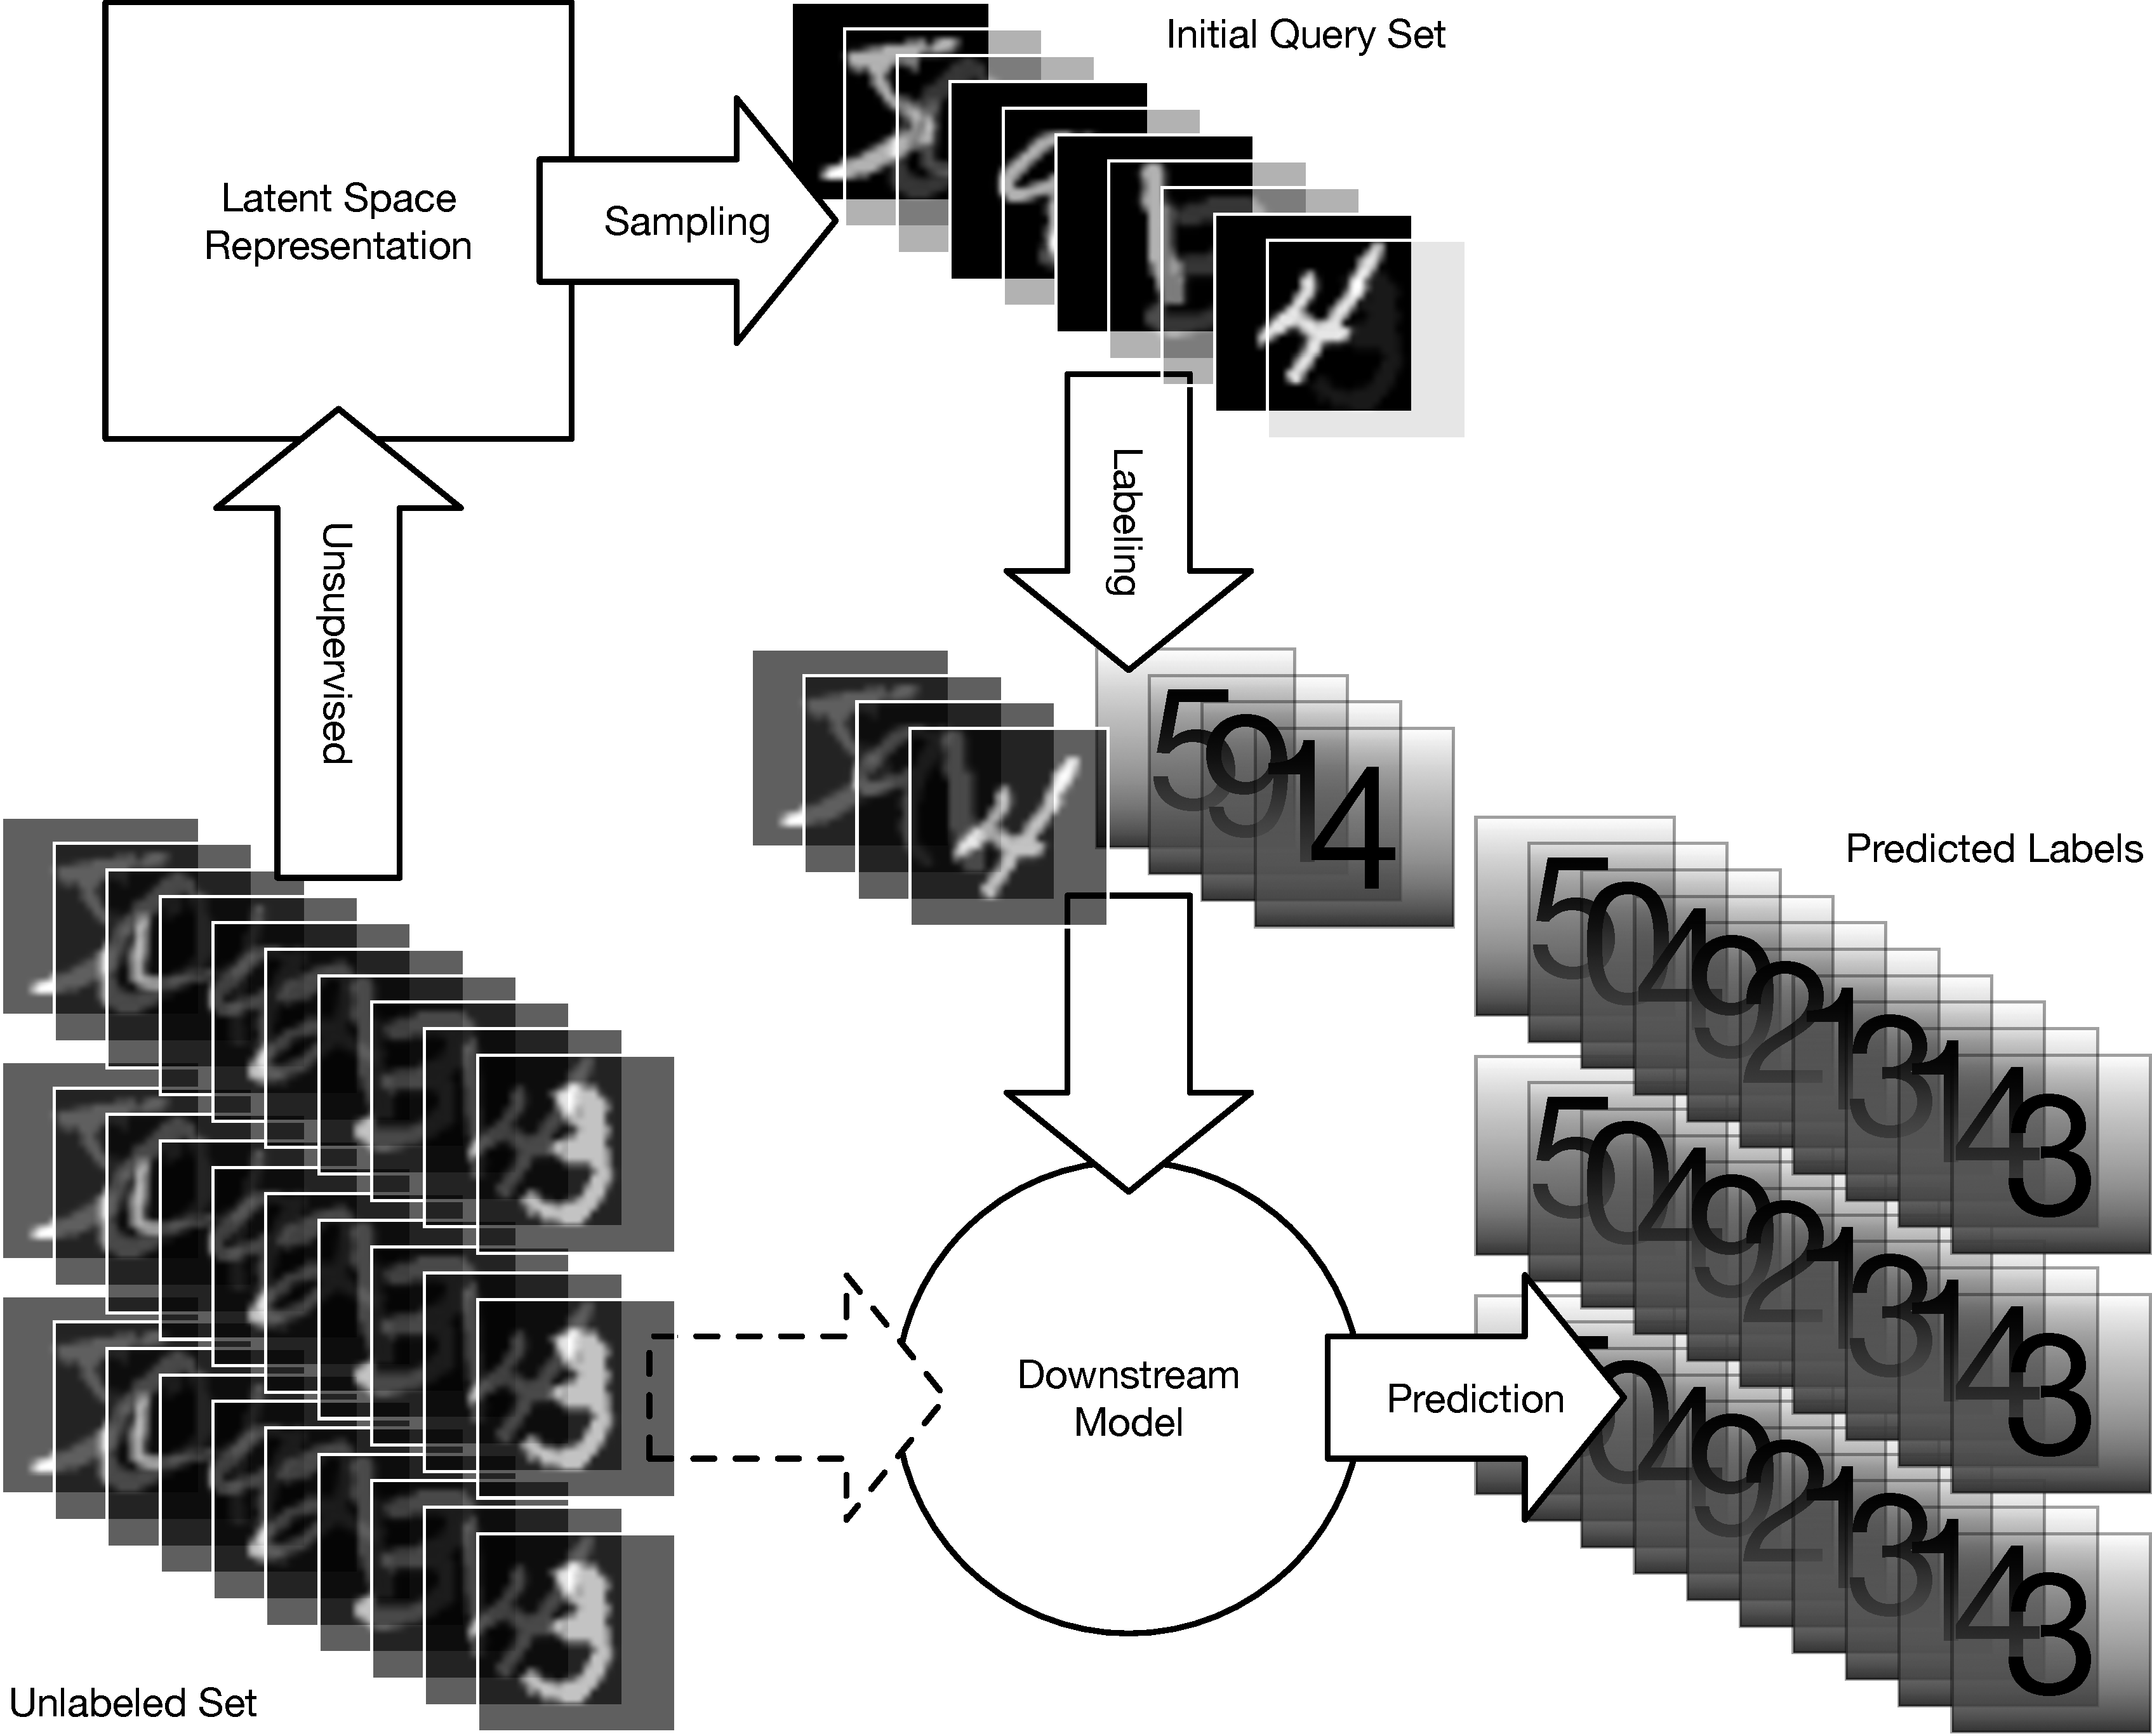
\includegraphics[width=\linewidth]{docs/query_selection}
  \caption{our initial query selection method (red) in relation to a downstream
    learning method (blue) like active or semi-supervised learning.}
  \label{fig:overview}
\end{figure}

Our method for initial query selection relies first on an AE to learn an
encoding in latent space and second on a sampling strategy in that latent
space. Although we restrict the latent space to $\mathbb{R}^2$ in our
experiments (for the sake of visualization and understanding), we discuss here
the method for a general latent space $\mathbb{R}^L$. To that end, we consider a
set of images $\mat{X} = \{\vec{x}_i\}_{i=1}^N$, where $N$ is the number of
examples, and their encoding matrix $\mat{Z} \in \mathbb{R}^{N\times L}$. We
refer to each AE's encoder function
$f_{\vec{\theta}} : \mathbb{R}^D \rightarrow \mathbb{R}^L$ and decoder
$g_{\vec{\phi}} : \mathbb{R}^L \rightarrow \mathbb{R}^D$ where $D$ is the
dimensionality of each input image $\vec{x}$, and $\vec{\theta}$ and
$\vec{\phi}$ are parameter vectors for each model.

\subsection{Auto-encoder Architectures}
\label{sec:auto-encod-arch}

We decided to explore latent space representations learned by an AE in large
part because of the opportunity for shared network design. The encoder part of
any auto-encoder can be reformatted as a classifier by changing the
representation layer to a prediction layer and the loss function to categorical
cross-entropy. This also allows for transfer learning knowledge between the AE
and the classifier, although that is beyond the scope of this paper.

We explore the representations learned by three AE types: a Convolutional
Auto-encoder (CAE), a Variational Auto-encoder (VAE), and a somewhat novel
``t-SNE Style'' AE. Although the CAE is the only AE with ``Convolutional'' in
its name, each type does in fact use both convolution layers and transpose
convolution layers for encoding and decoding, with the main differences between
types being the representation layer and loss function.

\subsubsection{Convolutional Auto-encoder}
\label{sec:conv-auto-encod}

Our CAE consists of 28 layers. Inspired by the design in Krizhevsky \emph{et
  al.}, each layer uses the $ReLU$ activation function and employs zero-padding
to maintain image dimensions unless otherwise noted
\cite{krizhevsky_imagenet_2012, nair_rectified_nodate}. The first three layers
of the encoder $f_{\vec{\theta}}$ apply convolutions with $64$ kernels of shape
$3\times 3$. A $2\times 2$ max-pooling follows, reducing image size to
$14\times 14$. We apply another three convolution layers, this time with $32$
kernels each, along with a second $2\times 2$ max-pool, and three more
convolution layers with $32$ kernels each. We flatten the resulting
$7 \times 7 \times 32$ image and feed it through two $1024$-node fully connected
layers. Next, the representation layer uses $2$ fully-connected nodes with no
activation function. The activation at this layer constitutes the encoding
$z = g_{\vec{\phi}}(x)$ of the input image $\vec{x}$.

The decoder $g_{\vec{\phi}}$ emulates this design, feeding the representation
$z$ through the same layers in reverse order (without tying weights). In place
of each max-pool layer, we use a $2\times 2$ transpose convolution with a stride
of $2$ to increase image dimensions. Finally, a $1\times 1$ convolution layer
outputs the reconstructed image $g_{\vec{\phi}}(z)$. We use a simple MSE loss
between the original image $\vec{x}$ and the reconstruction
\begin{equation}
  \label{eq:1}
  \mathcal{L}_{\text{CAE}}(\vec{\theta}, \vec{\phi};\vec{x}) =
  ||g_{\vec{\phi}}(f_{\vec{\theta}}(\vec{x})) - \vec{x}||^2
\end{equation}
and take the mean over each batch.

\subsubsection{Variational Auto-encoder}
\label{sec:vari-auto-encod}

Our VAE uses the same basic structure while following conventional design for
VAEs, a full discussion of which is beyond the scope of this
paper. \cite{kingma_auto-encoding_2013}. In place of the CAE's representational
layer, we use $2$ fully-connected nodes to represent $\vec{\mu}_z$, taken as $z$
for the encoding, and a further $2$ nodes to represent
$\log(\vec{\sigma}_z)$. We draw the input to the decoder from a desired normal
distribution so that
\begin{equation}
  \label{eq:3}
  f_{\vec{\theta}} =
  \begin{cases}
    \vec{\mu}_z + \epsilon \vec{\sigma}_z & \text{training} \\
    \vec{\mu}_z & \text{else}
  \end{cases}
\end{equation}
where $\epsilon \sim \mathcal{N}(0,1)$ for every batch.

The loss used by VAEs merits its own discussion, but we present a brief summary
here. Variational auto-encoding presumes that some ``true'' latent-space
encoding has a prior distribution $p(\vec{z})$, which we take as a standard
normal distribution. The VAE approximates this posterior $p(\vec{z} | \vec{x})$
of $p$ with $q(\vec{z} | \vec{x})$ by minimizing the Kullback-Leibler divergence
between the two. Minimizing this quantity directly turns out to be
computationally intractible, so VAEs maximize the Evidence Lower BOund:
\begin{equation}
  \label{eq:2}
  \begin{split}
    \elbo(\vec{x}) =
    & \mathbb{E}\left[q(\vec{z}|\vec{x})\log p(\vec{x}|\vec{z})\right] \\
    & - D_{\text{KL}}\left(q(\vec{z}|\vec{x})||p(\vec{z})\right)
  \end{split}
\end{equation}
We can convert Equation~\ref{eq:2}, which concerns the probability model of
VAEs, into a loss function for encoders and decoders, by noting the resemblance
of $q(\vec{z}|\vec{x})$ to our encoder $f_{\vec{\theta}}(x)$ and
$q(\vec{x}|\vec{z})$ to our decoder $g_{\vec{\phi}}(z)$. We negate and expand
Equation~\ref{eq:2} to obtain the loss
\begin{equation}
  \label{eq:4}
  \begin{split}
    \mathcal{L}_{\text{VAE}}(\vec{\theta}, \vec{\phi};\vec{x}) =
    & \bce(\vec{x},g_{\vec{\phi}}(f_{\vec{\theta}}(x))) \\
    & - \frac{1}{2}\mathbb{E}\left[1 + \log(\vec{\sigma}_z) - \vec{\mu}_z^2 -
      \vec{\sigma}_z \right]
  \end{split}
\end{equation}
where $\vec{\mu}_z$ and $\log(\vec{\sigma}_z)$ are taken directly from
activations in the representation layer and $\bce$ and $\mathbb{E}$ denote the
binary cross entropy and mean, respectively, over each batch.

\subsubsection{``t-SNE Style'' Auto-encoder}
\label{sec:t-sne-style}

As implied by the name, our ``t-SNE Style'' AE emulates the behavior of a t-SNE
embedding in its representational layer \cite{maaten_learning_2009}. It uses the
same architecture as the CAE in Section~\ref{sec:conv-auto-encod} with a
different loss function that incorporates the matrix of representations
$\mat{Z}_B$ over each batch $B$. Recall the t-SNE relies on the conditional
probabilities
\begin{equation}
  \label{eq:5}
  p_{i|j} =
  \begin{cases}
    \frac{\exp(-||\vec{x}_i - \vec{x}_j||^2 / 2\sigma_i^2)}
    {\sum_{k\neq i}\exp(-||\vec{x}_i - \vec{x}_k||^2 / 2\sigma_i^2)}
    & i \neq j \\
    0 & i = j
  \end{cases}
\end{equation}
which we take over each batch, tuning each $\sigma_i$ to match the desired
perplexity. The joint probabilities are then
$p_{ij} = (p_{i|j} + p_{j|i})/2|B|$. We also define a joint distribution over
the representations:
\begin{equation}
  \label{eq:7}
  q_{ij} = \frac%
  {\left(1 + ||f_{\vec{\theta}}(\vec{x}_i) -
      f_{\vec{\theta}}(\vec{x}_j)||^2\right)^{-1}} %
  {\sum_{k\neq l} \left(1 + ||f_{\vec{\theta}}(\vec{x}_k) -
      f_{\vec{\theta}}(\vec{x}_l)||^2\right)^{-1}}
\end{equation}
and incorporate the KL divergence between these two distributions in our
loss. We have
\begin{equation}
  \label{eq:6}
  \begin{split}
    \mathcal{L}_{\text{t-SNE Style}}(\vec{\theta}, \vec{\phi};\vec{x})
    & = \bce(\vec{x},g_{\vec{\phi}}(f_{\vec{\theta}}(x))) \\
    & + \sum_i \sum_j p_{ji} \log \left( \frac{p_{ji}}{q_{ji}} \right)
  \end{split}
\end{equation}
where each summation is over the current batch.

\subsection{Sampling Strategies}
\label{sec:sampling-strategies}

Once we obtain the latent space representation $Z$ of data points $X$, the
question remains of how best to sample $Z$. In this paper, we explore four
options that rely on specific probability distributions in the latent space,
approximating samples taken from these distributions. Two of these options rely
on a hierarchical clustering to capture the natural clustering of points in the
latent space \cite{johnson_hierarchical_1967}.

Algorithm~\ref{alg:sampling} shows how a distribution (or set of distributions
on each cluster) can be approximately sampled from while still selecting
original data points. Our strategies are as follows:
\begin{itemize}
\item ``Uniform'' uses a uniform distribution over $Z$
  \[p = \unif(\min(Z), \max(Z)).\]
\item ``Multi-normal'' fits a mutlivariate normal distribution to $Z$, using
  \[p = \mathcal{N}(\mathbb{E}(Z), \cov(Z)).\]
\item ``Uniform Cluster'' uses the uniform distribution over each cluster
  \[p_S = \unif(\min(Z_S), \max(Z_S)).\]
\item ``Multi-normal'' fits a mutlivariate normal distribution to each cluster
  $Z_S$, using \[p_S = \mathcal{N}(\mathbb{E}(Z_S), \cov(Z_S)).\]
\end{itemize}

We compare these strategies with two baseline sampling strategies. The first,
``Random,'' selects $n$ random examples from the dataset. The second
``AE-error,'' selects the $n$ examples with the highest average absolute error
$\mathbb{E}|\vec{x_i} - g_{\vec{\phi}}(f_{\vec{\theta}}(x_i))|$.

\begin{algorithm}
  \begin{algorithmic}[1]
    \Require \hfill %
    \begin{itemize}
    \item the encoding $Z \in \mathbb{R}^L$,
    \item clustering $\mathbf{S} = \{S_1 , \dots, S_C\}$ on $Z$,
    \item distributions
      $\{p_S : \mathbb{R}^L \rightarrow \mathbb{R}| S \in \mathbf{S}\}$, and
    \item distance threshold
      $t \in \mathbb{R}$, $n \in \mathbb{N}$.
    \end{itemize}

    \State $Q \gets \{\}$ %
    \For {Cluster $S \in \textbf{S}$} %
    \State $n_S \gets \round\left(n \frac{|S|}{N}\right) $ %
    \State $Q_S \gets \{\} $ %
    \While {$|Q_S| < n_S$} %
    \State Draw $z \sim p_S$ %
    \For {$i \in S$} \Comment the $i$th row of $Z$, in cluster $S$ %
    \If {$||z - z_i||_2 < t$} %
    \State $Q_S \gets Q_S \cup \{i\}$ %
    \EndIf %
    \EndFor %
    \EndWhile %
    \State $Q \gets Q \cup Q_S$ %
    \EndFor %
    \State \Return $Q$ %
  \end{algorithmic}
  \caption{Select examples from the clustered encoding $Z$ according to a
    distribution $p_S$ on each cluster $S$. Applies to sampling strategies
    without clustering if $\mathbf{S} = \{[N]\}$.}
  \label{alg:sampling}
\end{algorithm}

\section{Results}
\label{sec:results}

We present our results on two versions of the MNIST dataset, the original and a
second, unbalanced version \cite{lecun_mnist_2010}. In all our experiments, we
use the first $N = 50000$ examples for AE training and sampling, with the
remaining $20000$ examples reserved for validation and test sets. We use two
versions of MNIST in order to demonstrate the main advantage of latent space
sampling when starting with no labels. For a balanced dataset with equal
representation from each class, taking a random subset of $X$ results in a
sufficiently balanced query set even for relatively small a sample size. We
created an unbalanced version of MNIST by increasing the representation of each
even digit by $2000$ and removing the same number of examples for each odd
digit. To create new examples, we apply a small translation and rotation to
randomly selected originals of the same class. These changes do not affect the
validation and test sets. For each dataset, we experimented with two sample or
query set sizes, $n=1000$ and $n=100$.

% Because of the $L = 2$ constraint, our latent space encodings displayed
% significant overlap between the original classes in the data. Typically, 0s and
% 1s were well separated, but 4s and 9s often overlapped, along with 3s and
% 8s. Figure~\ref{fig:vae-encodings} shows the encoding of the training set
% learned by our VAE on the unbalanced MNIST dataset, demonstrating this overlap
% property well. Additionally, this figure illustrates some of the difficulties
% associated with sampling the latent space. Well-separated classes like 0 and 1
% occupy a larger region, and so sampling strategies that used a single
% distribution generally contained much more representation from these classes
% than the rest, while classes that overlapped had less representation in the
% sample, especially for any ``Uniform'' sampling strategy.

To evaluate our latent space representations and sampling strategies
quantitatively, we train a convolutional neural network (CNN) with the same
design as the encoders in Section~\ref{sec:auto-encod-arch}. We train each CNN
for 50 epochs on the 1000-example query sets and 500 epochs on the 100-examples
sets. In this way, each classifier has an identical number of update steps for
training. Figure~\ref{fig:classifier-accs} shows the validation-set accuracies
of a classifier as it trains on the query set of 100 examples from the
unbalanced MNIST data. As is clear, the ``Multi-normal Cluster'' sampling
strategy outperforms random sampling, likely because it has a much more balance
distribution of classes. Classifiers that used query sets with other sampling
strategies struggled to train.

As can be seen in Table~\ref{tab:results}, this was not the case for our other
experiments. Especially when query sets sampled from the original MNIST data,
random sampling outperformed or nearly equaled every other strategy. This is to
be expected. When sampling from random distributions, as we do, the
already class-balanced distribution of the original dataset is optimal. The
performance of ``Multi-normal Cluster'' sampling is encouraging in this light
because, although it fails to do better than random sampling, it recovers the
same balance in its sampling. Our experiments with the unbalanced dataset
confirm this suspicion.

\begin{figure}
  \centering
  \subfloat[]{
    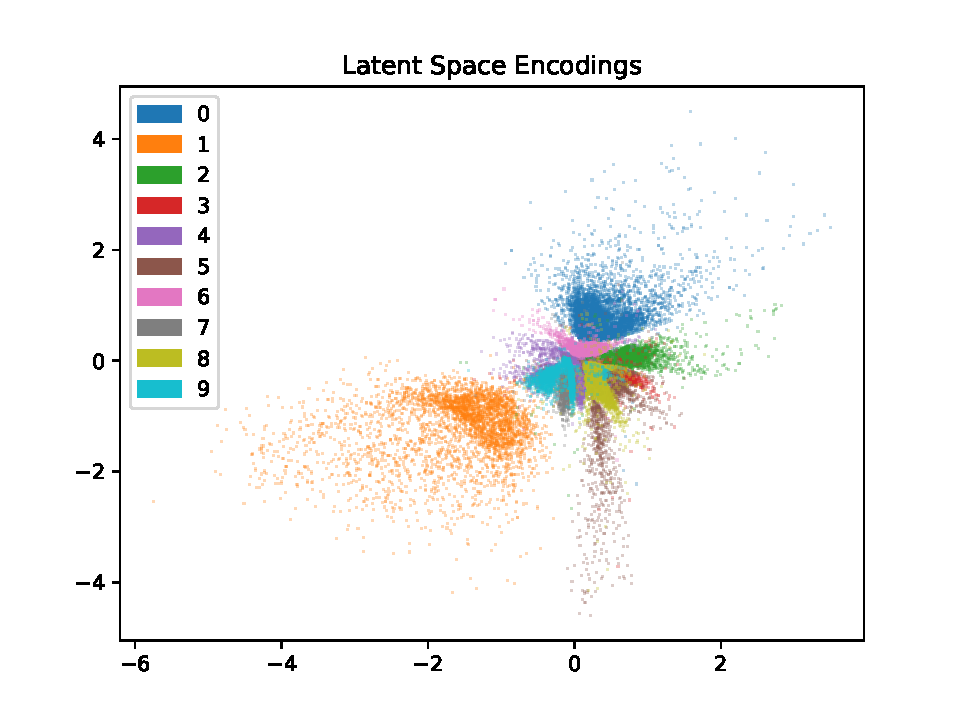
\includegraphics[width=\linewidth]
    {models/unbalanced_mnist_vae_e300_L2_b64/encodings}
    \label{fig:vae-encodings}
  } \\
  \subfloat[]{
    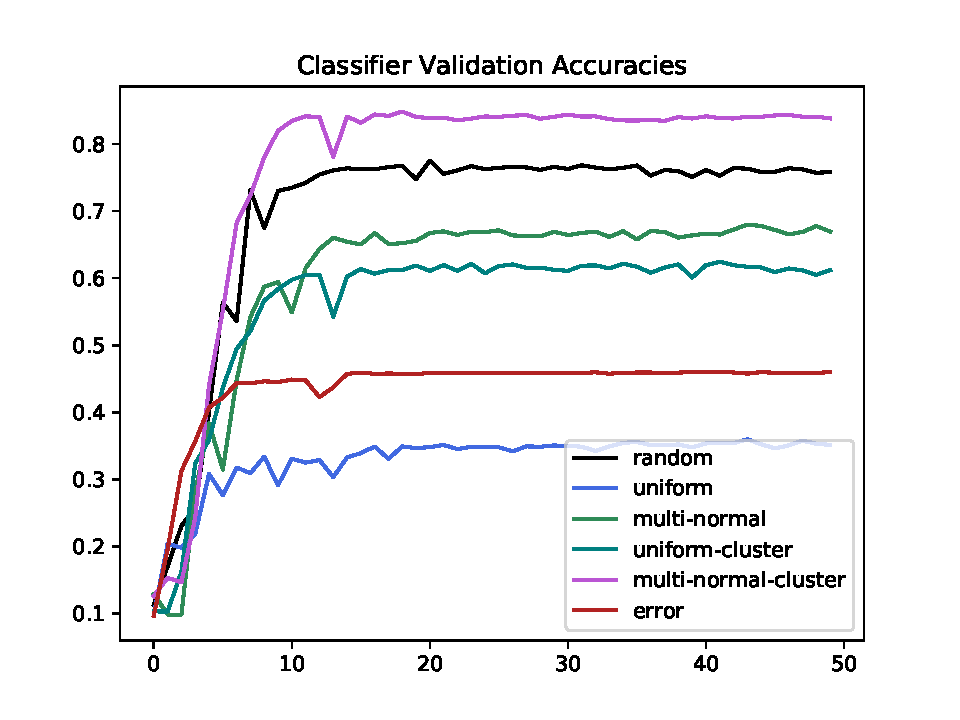
\includegraphics[width=\linewidth]
    {models/unbalanced_mnist_vae_e300_L2_b64/classifier_val_accs_100}
    \label{fig:classifier-accs}
  }
  \caption{(\ref{fig:vae-encodings}) shows latent-space encoding for the
    unbalanced MNIST training set using a VAE. (\ref{fig:classifier-losses})
    shows the validation set loss during training for a classifier on a training
    set of size 100. (Epoch count in 10s.)}
  \label{fig:unbalanced-mnist-results}
\end{figure}

\begin{table*}[]
  \centering
  \begin{tabular}{|l|l|m{3em} m{3em}|m{3em} m{3em}|}
    \hline
    \multicolumn{1}{|c|}{AE Type} & \multicolumn{1}{|c|}{Sampling Strategy}
    & \multicolumn{2}{|c|}{Original MNIST} & \multicolumn{2}{|c|}{Unbalanced MNIST} \\
    & & \multicolumn{1}{|c}{1000} & \multicolumn{1}{c|}{100} & \multicolumn{1}{|c}{1000} & \multicolumn{1}{c|}{100} \\
    \hline
    --- & Random & $94.0_{\pm .2}$ & $80.9_{\pm 1.8}$ & $92.6_{\pm .4}$ & $76.6_{\pm .6}$\\
    \hline
    --- & AE-error & $93.8_{\pm .3}$ & $76.6_{\pm .4}$ & $57.8_{\pm .2}$ & $46.4_{\pm .2}$ \\
    \hline
    \multirow{4}{4em}{CAE}
    & Uniform
      & 72.7 & 38.1 & 62.9 & 44.6 \\
    & Multi-normal
      & 93.1 & 70.3 & 90.5 & 66.3 \\
    & Uniform Cluster
      & 89.6 & 71.6 & 89.2 & 71.5 \\
    & Multi-normal Cluster
      & 94.4 & 80.9 & 92.8 & 79.6 \\
    \hline
    \multirow{4}{4em}{VAE}
    & Uniform
      & 68.2 & 38.8 & 62.4 & 35.3 \\
    & Multi-normal
      & 92.1 & 69.9 & 91.7 & 66.5 \\
    & Uniform Cluster
      & 86.1 & 67.3 & 86.8 & 62.1 \\
    & Multi-Normal Cluster
      & 94.3 & \textbf{82.9} & 92.3 & \textbf{85.0} \\
    \hline
    \multirow{4}{4em}{t-SNE Style}
    & Uniform
      & 69.3 & 56.6 & 85.7 & 53.0 \\
    & Multi-normal
      & 93.6 & 82.3 & 91.7 & 77.0 \\
    & Uniform Cluster
      & 87.3 & 71.6 & 91.6 & 76.6 \\
    & Multi-normal Cluster
      & 94.4 & 78.9 & 92.4 & 75.9 \\
    \hline
  \end{tabular}
  \caption{Test-set accuracies (\%) for a classifier trained on query sets from
    both the balanced and unbalanced MNIST data. As can be seen, the advantage
    of latent space sampling is most apparent when the original data is
    unbalanced and the sample size is small enough to reflect it.}
  \label{tab:results}
\end{table*}

\section{Discussion}
\label{sec:discussion}

The success of our ``Multi-normal Cluster'' sampling strategy using the VAE
representation is encouraging, but many areas remain open to inquiry. One could
explore higher dimensional latent spaces, for instance, and while this could
improve performance, we argue that it offers little insight into the underlying
problems of initial query selection. Those problems consist of two main
questions: ``What is the best space to sample from?'' and ``What is the best
sampling strategy for that space?'' Unfortunately, one cannot investigate each
question separately. Consider the poor performance of uniform-distribution-based
samplers in our experiments, which does not necessarily extend to every latent
space representation of the data. While the similarity of AEs to the supervised
models used in downstream approaches motivated their use in our experiments,
other embedding methods may yield more effective performance when combined with
our sampling strategies. Additionally, more nuanced sampling strategies could
prove effective for a variety of latent space representations.

Although we used distribution-based sampling strategies in our experiments, we
believe that deterministic approaches could be more reliable. Future work should
identify examples which result in an initial query set balanced not only with
respect to classes, like our random sampling baseline on original MNIST, but
also with respect to different forms classes. The same digit may be drawn in
different styles, for example, each of which should be present in an initial
query set.

\section{Conclusions}
\label{sec:conclusion}

We have shown the potential for latent space sampling to identify a useful
initial query set, especially from an unbalanced data. We have shown the
effectiveness (or ineffectiveness) of four simple sampling strategies on three
types of latent spaces compared to two simple baselines: random selection and
error-based selection. In particular, we have compared the test-set accuracies
of a classifier trained on each query set. The success of cluster-based methods
in this space calls for further exploration of cluster-based sampling
strategies.

\section{Acknowledgements}
\label{sec:acknowledgements}

Thanks to Gordon Kindlmann for computational resources. Implementation and
sampling strategies are original work, as well as the t-SNE Style AE.

\newpage
\eightpt
\bibliographystyle{IEEEtran}

\bibliography{report}

\end{document}

%%% Local Variables:
%%% mode: latex
%%% TeX-master: t
%%% End:
